% Chapter 4

\chapter{Inference of mutual information} % Main chapter title

\label{Chapter4} % For referencing the chapter elsewhere, use \ref{Chapter1} 

\section{Motivation}

As we discussed in the introduction, the mutual information $I(X; Y)$
provides one method for the supervised evaluation of representations.
Recall that Shannon's mutual information $I(X; Y)$ is fundamentally a
measure of dependence between random variables $X$ and $Y$, defined as
\[
I(X;Y) = \int p(x, y) \log \frac{p(x, y)}{p(x)p(y)}dxdy.
\]
Various properties of $I(\vec{g}(\vec{Z}); Y)$, such as sensitivity to
nonlinear relationships, symmetry, and invariance to bijective
transformations, make it ideal for quantifying the information between
a representation of an input vector $\vec{g}(\vec{Z})$ and a (possibly
vector-valued) response $Y$.  

However, current methods estimating mutual information for
high-dimensional data either require large and over-parameterized
generative models, or work only for discrete responses.  For
continuous $(X, Y)$, one can tractably estimate mutual information by
assuming a multivariate Gaussian model: however, this approach
essentially assumes a linear relationship between the input and
output, and hence fails to quantify nonlinear dependencies.
Meanwhile, in the case of a discrete response $Y$, one can obtain a
lower bound on the mutual information by using the confusion matrix of
a classifier.  This is the most popular approach for estimating mutual
information in neuroimaging studies, but suffers from known
shortcomings (\cite{Gastpar2009}, \cite{QuianQuiroga2009}).  The idea
of linking classification performance to mutual information dates back
to the beginnings of information theory: Shannon's original motivation
was to characterize the minimum achievable error probability of a
noisy communication channel.  More explicitly, Fano's inequality
(\cite{fano1961transmission}) provides a lower bound on mutual
information in relation to the optimal prediction error, or Bayes
error.  Fano's inequality can be further refined to obtain a tighter
lower bound on mutual information (\cite{tebbe1968uncertainty}.)
However, a shortcoming to all of these classification-based approaches
is that if $Y$ is not already discrete, the discretization of the
response $Y$ necessarily loses information.

In this chapter, we develop an analogue of Fano's inequality for the
\emph{identification task}, rather than the classification task, which
can therefore be applied to the case of a continuous response $Y$.  In
this way, we derive a new machine-learning based estimator of mutual
information $I(X; Y)$ which can be applied without the need to
discretize a continuous response.

As we saw in Chapter 2, the identification task is highly related to
the randomized classification framework.  Therefore, we analyse the
identification risk by means of the $k$-class average Bayes accuracy,
which provides an upper bound to identification accuracy.  Our main
theoretical contributions are (i) the derivation of a tight lower
bound on mutual information as a function of $k$-class average Bayes
accuracy, and (ii) the derivation of an asymptotic relationship
between the $K$-class average Bayes accuracy and the mutual
information. Our method therefore estimates the $K$-class Bayes
identification accuracy to be translated into estimate of the mutual
information.

Our method complements the collection of existing approaches for
estimating mutual information in the sense that it allows the
leveraging of different kinds of prior assumptions than ones
previously considered in the literature.  Our target application is
when the relationship between the random variables $(X, Y)$ is
well-described by a parametric regression model $\E[Y|X=x] =
f_\theta(x)$.  An important special case is when a \emph{sparse}
relationship exists between the predictor and response.  As we will
demonstrate, exploiting sparsity assumptions can vastly improve the
efficiency of estimation in high-dimensional settings.

The rest of the chapter is organized as follows.  Section
\ref{sec:ch4_theory} establishes the theoretical results linking
average Bayes accuracy and mutual information, and section
\ref{sec:ch4_estimation} describes our proposed identification-based
estimator of mutual information based on the theory.  We present one
simulation example in section \ref{sec:ch4_simulation}, but will we
also see some real data applications in the next chapter.
%, where the
%estimator developed here is compared to an alternative estimator,
%which is based on high-dimensional asymptotics.

\section{Average Bayes accuracy and Mutual information}\label{sec:ch4_theory}

\subsection{Problem formulation and result}

Let $\mathcal{P}$ denote the collection of all joint densities $p(x,
y)$ on finite-dimensional Euclidean space.  For $\iota \in [0,\infty)$
define $C_k(\iota)$ to be the largest $k$-class average Bayes error
attained by any distribution $p(x,y)$ with mutual information not
exceeding $\iota$:
\[
C_k(\iota) = \sup_{p \in \mathcal{P}: \text{I}[p(x,y)] \leq \iota} \text{ABA}_k[p(x,y)].
\]
A priori, $C_k(\iota)$ exists since $\text{ABA}_k$ is bounded between
0 and 1.  Furthermore, $C_k$ is nondecreasing since the domain of the
supremum is monotonically increasing with $\iota$.

It follows that for any density $p(x,
y)$, we have
\[
\text{ABA}_k[p(x,y)] \leq C_k(\text{I}[p(x,y)]).
\]
Hence $C_k$ provides an upper bound for average Bayes error in terms of mutual information.

Conversely we have
\[
\text{I}[p(x,y)] \geq C^{-1}_k(\text{ABA}_k[p(x,y)])
\]
so that $C^{-1}_k$ provides a lower bound for mutual information in terms of average Bayes error.

On the other hand, there is no nontrivial \emph{lower} bound for average Bayes error in terms of mutual information,
nor upper bound for mutual information in terms of average Bayes error, since
\[
\inf_{p \in \mathcal{P}: \text{I}[p(x,y)] \leq \iota} \text{ABA}_k[p(x,y)] = \frac{1}{k}.
\]
regardless of $\iota$.

The goal of this work is to attempt to compute or approximate the functions $C_k$ and $C_k^{-1}$.

In the following sections we determine the value of $C_k(\iota)$,
leading to the following result.

\begin{theorem}\label{theorem:Cunif}
For any $\iota > 0$, there exists $c_\iota \geq 0$ such that defining
\[
Q_c(t) = \frac{\exp[ct^{k-1}]}{\int_0^1 \exp[ct^{k-1}]},
\]
we have
\[
\int_0^1 Q_{c_\iota}(t) \log Q_{c_\iota}(t) dt = \iota.
\]
Then,
\[
C_k(\iota) = \int_0^1 Q_{c_\iota}(t) t^{k-1} dt.
\]
\end{theorem}

We obtain this result by first reducing the problem to the case of
densities with uniform marginals, then doing the optimization over the
reduced space.

\subsection{Reduction}

Let $p(x, y)$ be a density supported on
$\mathcal{X} \times \mathcal{Y}$, where $\mathcal{X}$ is a subset of
$\mathbb{R}^{d_1}$ with a non-empty interior, and $\mathcal{Y}$ is a subset of
$\mathbb{R}^{d_2}$, also with non-empty interior, and such that $p(x)$ is uniform on $\mathcal{X}$
and $p(y)$ is uniform on $\mathcal{Y}$.

Now let $\mathcal{P}^{unif}$ denote the set of such distributions:
in other words, $\mathcal{P}^{unif}$ is the space of joint densities in Euclidean space
with uniform marginals over the marginal supports.
In this section, we prove that
\[
C_k(\iota) =\sup_{p \in \mathcal{P}: \text{I}[p(x,y)] \leq \iota} \text{ABA}_k[p(x,y)] = 
\sup_{p \in \mathcal{P}^{unif}: \text{I}[p(x,y)] \leq \iota} \text{ABA}_k[p(x,y)],
\]
thus reducing the problem of optimizing over the space of all
densities to the problem of optimizing over densities with uniform
marginals.

Also define $\mathcal{P}^{bounded}$ to be the space of all densities $p(x, y)$ with finite-volume support.
Since uniform distributions can only be defined over sets of finite volume, we have
\[
\mathcal{P}^{unif} \subset \mathcal{P}^{bounded} \subset \mathcal{P}.
\]

Therefore, it is necessary to first show that
\[
\sup_{p \in \mathcal{P}: \text{I}[p(x,y)] \leq \iota} \text{ABA}_k[p(x,y)] = 
\sup_{p \in \mathcal{P}^{bounded}: \text{I}[p(x,y)] \leq \iota} \text{ABA}_k[p(x,y)].
\]

This is accomplished via the following lemma.

\begin{lemma}\label{lemma:truncation} (Truncation).
Let $p(x, y)$ be a density on
$\mathbb{R}^{d_x} \times \mathbb{R}^{d_y}$.  For all $\epsilon > 0$,
there exists a subset $\mathcal{X} \subset \mathbb{R}^{d_x}$ with
finite volume with respect to $d_x$-dimensional Lesbegue measure, and
a subset $\mathcal{Y} \subset \mathbb{R}^{d_y}$ with finite volume
with respect to $d_y$-dimensional Lesbegue measure, such that defining
\[
\tilde{p}(x, y) = \frac{I\{(x,y) \in \mathcal{X}\times \mathcal{Y}\} }{\int_{\mathcal{X} \times \mathcal{Y}} p(x,y) dx dy} p(x,y),
\]
we have
\[
|\text{I}[p] - \text{I}[\tilde{p}]| < \epsilon
\]
and
\[
|\text{ABA}_k[p] - \text{ABA}_k[\tilde{p}]| < \epsilon.
\]
\end{lemma}

\textbf{Proof.}
Recall the definition of the Shannon entropy $H$:
\[
\text{H}[p(x)] = - \int p(x) \log p(x) dx.
\]
It is a well-known in information theory that
\[
\text{I}[p(x, y)] = \text{H}[p(x)] + \text{H}[p(y)] - \text{H}[p(x, y)].
\]
There exists a sequence $(\mathcal{X}_i, \mathcal{Y}_i)_{i=1}^\infty$
where $(\mathcal{X}_i)_{i=1}^\infty$ is an increasing sequence of finite-volume subsets of $\mathbb{R}^{d_x}$
and $(\mathcal{Y}_i)_{i=1}^\infty$ is an increasing sequence of finite-volume subsets of $\mathbb{R}^{d_y}$,
and $\lim_{i \to \infty} \mathcal{X}_i = \mathbb{R}^{d_x}$, $\lim_{i \to \infty} \mathcal{Y}_j$.
Define
\[
\tilde{p}_i(x, y) = \frac{I\{(x,y) \in \mathcal{X}_i\times \mathcal{Y}_i\} }{\int_{\mathcal{X}_i \times \mathcal{Y}_i} p(x,y) dx dy} p(x,y)
\]
Note that $\tilde{p}_i$ gives the conditional distribution of $(X, Y)$
conditional on $(X, Y) \in \mathcal{X}_i \times \mathcal{Y}_i$. 
Furthermore, it is convenient to define $\tilde{p}_\infty = p$.
We can find some $i_1$, such that for all $i \geq i_1$, we have
\[
\left|\int_{x \notin \mathcal{X}_i} p(x) \log p(x) dx\right| < \frac{\epsilon}{6}
\]
\[
\left|\int_{y \notin \mathcal{Y}_i} p(y) \log p(y) dy\right| < \frac{\epsilon}{6}
\]
\[
\left|\int_{(x,y) \notin \mathcal{X}_i \times \mathcal{Y}_i} p(x, y) \log p(x, y) dx dy\right| < \frac{\epsilon}{6}
\]
and also such that
\[
-\log \left[\int_{x, y \in \mathcal{X}_i \times \mathcal{Y}_i} p(x, y) dx dy\right] < \frac{\epsilon}{2}
\]
Then, it follows that
\[
|\text{I}[p] - \text{I}[\tilde{p}_i]| < \epsilon
\]
for all $i \geq i_1$.

Now we turn to the analysis of average Bayes error.
Let $f_i$ denote the Bayes $k$-class classifier for $\tilde{p}_i(x, y)$
and
$f_\infty$ the Bayes $k$-class classifier for $p(x, y)$: recall that by definition,
\[
\text{ABA}_k[\tilde{p}_i] = \Pr_{\tilde{p}_i}[f_i(Y^{(1)},...,Y^{(k)}, X) = Y^{(1)}]
\]
where the probability is taken with respect to the joint distribution
of $Y^{(1)},\hdots, Y^{(k)}$ drawn from $\pi$, and $X$ drawn from the
conditional distribution $F_{Y^{(1)}}.$
Define
\[
\epsilon_i = \Pr_p[(Y^{(1)},...,Y^{(k)}, X)\notin \mathcal{Y}_i^k \times \mathcal{X}_i ];
\]
by continuity of probability we have $\lim_i \epsilon_i \to 0$.
We claim that
\[
|\text{ABA}_k[\tilde{p}_i] - \text{ABA}_k[p]| \leq \epsilon_i.
\]
Given the claim, the proof is completed by finding $i > i_1$ such that $\epsilon_i < \epsilon$,
and defining $\mathcal{X} = \mathcal{X}_i$, $\mathcal{Y} = \mathcal{Y}_i$.

Consider using $f_i$ to obtain a classification rule for $p(x, y)$:
define
\[
\tilde{f}_i = \begin{cases}f_i(y^{(1)},\hdots,y^{(k)}, x) & \text{ when } (y^{(1)},\hdots,y^{(k)}, x) \in \mathcal{X}_i^k \times \mathcal{Y}_i\\
0 & \text{ otherwise.} 
\end{cases}
\]
We have
\begin{align*}
\text{ABA}_k[p] =& \sup_f \Pr_p[f(Y^{(1)},\hdots,Y^{(k)}, X) = Y^{(1)}]
\\ \geq& 
\\=& (1-\epsilon_i)\Pr_p[f_i(Y^{(1)},\hdots,Y^{(k)}, X) = Y^{(1)}|(Y^{(1)},\hdots,Y^{(k)}, X)\in \mathcal{X}_i^k \times \mathcal{Y}_i]
\\&+ \epsilon_i \Pr_p[f_i(Y^{(1)},\hdots,Y^{(k)}, X) = Y^{(1)}|(Y^{(1)},\hdots,Y^{(k)}, X)\notin \mathcal{X}_i^k \times \mathcal{Y}_i]
\\=& (1-\epsilon_i)\Pr_{\tilde{p}}[f_i(Y^{(1)},\hdots,Y^{(k)}, X) = Y^{(1)}]
+ \epsilon_i 0
\\=& (1-\epsilon_i) \text{ABA}_k[\tilde{p}_i] \geq \text{ABA}_k[\tilde{p}_i] - \epsilon_i.
\end{align*}
In other words, when $\tilde{p}_i$ is close to $p$, the Bayes
classification rule for $\tilde{p}_i$ obtains close to the Bayes rate
when the data is generated under $p$.

Now consider the reverse scenario of using $f_p$ to perform
classification under $\tilde{p}_i$.  This is equivalent to generating
data under $p(x, y)$, performing classification using $f$, then only
evaluating classification accuracy conditional on $(Y^{(1)},...,Y^{(k)},
X)\in \mathcal{X}_i^k \times \mathcal{Y}_i$.  Therefore,

\begin{align*}
\text{ABA}_k[\tilde{p}_i] =& \sup_f \Pr_{\tilde{p}_i}[f(Y^{(1)},\hdots,Y^{(k)}, X) = Y^{(1)}]
\\\geq &  \Pr_{\tilde{p}_i}[f_i(Y^{(1)},\hdots,Y^{(k)}, X) = Y^{(1)}]
\\=& \Pr_p[f_i(Y^{(1)},\hdots,Y^{(k)}, X) = Y^{(1)}| (Y^{(1)},\hdots,Y^{(k)}, X)\in \mathcal{X}_i^k \times \mathcal{Y}_i]
\\=& \frac{1}{1-\epsilon_i} \Pr_p[I\{(X^{(1)},...,X^{(k)}, Y)\in \mathcal{X}_i^k \times \mathcal{Y}_i\} \text{ and }f_i(Y^{(1)},\hdots,Y^{(k)}, X) = Y^{(1)}]
\\\geq & \frac{1}{1-\epsilon_i} \left(1 - \Pr_p[I\{(Y^{(1)},...,Y^{(k)}, X)\notin \mathcal{X}_i^k \times \mathcal{Y}_i\}] - \Pr_p[f_p(Y^{(1)},\hdots,Y^{(k)}, X) \neq Y^{(1)}]]\right)
\\&= \frac{\text{ABA}_k[p] - \epsilon_i}{1-\epsilon_i} \geq \text{ABA}_k[p] - \epsilon_i.
\end{align*}
In other words, when $\tilde{p}_i$ is close to $p$, the Bayes
classification rule for $p$ obtains close to the Bayes rate when the
data is generated under $\tilde{p}_i$.

Combining the two directions gives $|\text{ABA}_k[\tilde{p}_i]
- \text{ABA}_k[p]| \leq \epsilon_i$, as claimed. $\Box$

One can go from bounded-volume sets to uniform distributions by adding
auxillary variables.  To illustrate the intution, consider a density
$p(x)$ on a set of bounded volume, $\mathcal{X}$.  Introduce a
variable $W$ such that conditional on $X = x$, we have $w$ uniform on
$[0, p(x)]$.  It follows that the joint density $p(x, w) = 1$ and is
supported on a set $\mathcal{X}' = \mathcal{X} \times [0,\infty]$.
Furthermore, $\mathcal{X}'$ is of bounded volume (in fact, of volume 1) since
\[
\int_{\mathcal{X}'} dx = \int_{\mathcal{X}'} p(x, w) dx = 1.
\]

Therefore, to accomplish the reduction from $\mathcal{P}$ to
$\mathcal{P}^{unif}$, we start with a density
$p(x,y) \in \mathcal{P}$, and using Lemma \ref{lemma:truncation},
find a suitable finite-volume truncation $\tilde{p}(x, y).$ Finally,
we introduce auxillary variables $w$ and $z$ so that the expanded
joint distribution $p(x, w, y, z)$ has uniform marginals $p(x, w)$ and
$p(y, z)$.  However, we still need to check that the introduction of
auxillary variables preserves the mutual information and average Bayes
error; this is the content of the next lemma.

\begin{lemma}
Suppose $X$, $Y$, $W$, $Z$ are continuous random variables, and that
$W\perp Y|Z$, $Z \perp X|Y$, and $W \perp Z|(X,Y)$.  Then,
\[
\text{I}[p(x, y)] = \text{I}[p((x,w), (y,z))]
\]
\end{lemma}
\textbf{Proof.}
Due to conditional independence relationships, we have
\[
p((x,w), (y,z)) = p(x,y)p(w|x)p(z|y).
\]

It follows that
\begin{align*}
\text{I}[p((x,w), (y,z))] &= \int dx dw dy dz  \ p(x,y)p(w|x)p(z|w) \log \frac{p((x,w), (y,z))}{p(x,w)p(y,z)}
\\&= \int dx dw dy dz \ p(x,y)p(w|x)p(z|w) \log \frac{p(x, y)p(w|x)p(z|y)}{p(x)p(y)p(w|x)p(z|y)}
\\&= \int dx dw dy dz \ p(x,y)p(w|x)p(z|w) \log \frac{p(x, y)}{p(x)p(y)}
\\&= \int dx dy \ p(x,y) \log \frac{p(x, y)}{p(x)p(y)} = \text{I}[p(x,y)].
\end{align*}

Also,
\begin{align*}
\text{ABA}_k[p((x,w),(y,z))] 
&= \int \left[\prod_{i=1}^k p(x_i, w_i) dx_i dw_i \right] \int dy dz \ \max_i p(y,z|x_i, w_i).
\\&= \int \left[\prod_{i=1}^k p(x_i, w_i) dx_i dw_i \right] \int dy \ \max_i p(y|x_i) \int dz \ p(z|y).
\\&= \int \left[\prod_{i=1}^k p(x_i) dx_i \right] \left[\prod_{i=1}^k \int dw_i p(w_i|x_i)\right] \int dy \ \max_i p(y|x_i)
\\&= \text{ABA}_k[p(x,y)].
\end{align*}

$\Box$


Combining these lemmas gives the needed reduction, given by the following theorem.

\begin{theorem}\label{theorem:reduction} (Reduction.)
\[
\sup_{p \in \mathcal{P}: \text{I}[p(x,y)] \leq \iota} \text{ABA}_k[p(x,y)] = 
\sup_{p \in \mathcal{P}^{unif}: \text{I}[p(x,y)] \leq \iota} \text{ABA}_k[p(x,y)].
\]
\end{theorem}

The proof is trivial given the previous two lemmas.

%\subsection{Optimization}

%Having reduced the problem to an optimization over $\mathcal{P}^{unif}$,
%in this section we use variational calculus to find the global optimum to the optimization problem
%\[
%\text{maximize}_{p \in \mathcal{P}^{unif}: \text{I}[p(x,y)] \leq \iota} \text{ABA}_k[p(x,y)]
%\]

\subsection{Proof of theorem}

\textbf{Proof of theorem \ref{theorem:Cunif}}

Using Theorem \ref{theorem:reduction}, we have
\[
C_k(\iota) = \sup_{p \in \mathcal{P}^{unif}: \text{I}[p(x,y)] \leq \iota} \text{ABA}_k[p(x,y)].
\]

Define $\sigma(\iota) = \int_0^1 Q_{c_\iota}(t) t^{k-1} dt$: our goal is to
establish that $C_k(\iota) = \sigma(\iota)$.  
Note that $\sigma(\iota)$
is the same function which appears in Lemma \ref{lemma:concave} and
the same bound as established in Lemma \ref{lemma:variational}.

Define the density $p_\iota(x, y)$ where
\[
p_\iota(x, y) = \begin{cases}
g_\iota(y - x) & \text{ for } x\geq y\\
g_\iota(1 + y - x) & \text{ for } x < y
\end{cases}
\]
where
\[
g_\iota(x) = \frac{d}{dx}G_\iota(x)
\]
and $G_\iota$ is the inverse of $Q_c$.

One can verify that $\text{I}[p_\iota] = \iota$, and 
\[
\text{ABA}_k[p] = \int_0^1 Q_{c_\iota}(t) t^{k-1} dt.
\]

This establishes that
\[
C_k(\iota) \geq \int_0^1 Q_{c_\iota}(t) t^{k-1} dt.
\]
It remains to show that for all $p \in \mathcal{P}^{unif}$ with
$\text{I}[p] \leq \iota$, that $\text{ABA}_k[p] \leq \text{ABA}_k[p_\iota]$.

Take $p \in \mathcal{P}^{unif}$ such that $\text{I}[p] \leq \iota$.
Letting $Y^{(1)},...,Y^{(k)} \sim \text{Unif}[0,1]$, and $X \sim \text{Unif}[0,1]$ define $Z_i(x) = p(x|Y_i)$.
We have $\E(Z_1(x))$ and,
\[
\text{I}[p(x,y)] = \E(Z_1(X) \log Z_1(X))
\]
while
\[
\text{ABA}_k[p(x,y)] = k^{-1}\E(\max_i Z_i(X)).
\]

Letting $G_x$ be the distribution of $Z(x)$, we have
\[
E[G_x] = 1
\]
\[
\text{I}[p(x,y)] = \E(I[G_X])
\]
\[
\text{ABA}_k[p(x,y)] = \E(\psi_k[G_X])
\]
where the expectation is taken over $X \sim \text{Unif}[0,1]$ and
where $E[G]$, $I[G]$, and $\psi_k[G]$ are defined as in
Lemma \ref{lemma:variational}.

Define the random variable $J = I[G_Y]$.
We have
\begin{align*}
\text{ABA}_k[p(x,y)] &= \E(\psi_k[G_X])
\\&= \int_0^1 \psi_k[G_X] dy
\\&\leq \int_0^1 \left(\sup_{G: I[G] \leq I[G_x]} \psi_k[G]\right) dy
\\&= \int_0^1 \sigma(I[G_x]) dy = \E[\sigma(J)].
\end{align*}
Now, since $f$ is concave by Lemma \ref{lemma:concave},
we can apply Jensen's inequality to conclude that
\[
\text{ABA}_k[p(x,y)] = \E[\sigma(J)] \leq \sigma(\E[J]) = \sigma(\iota),
\]
which completes the proof. $\Box$



\section{Estimation}\label{sec:ch4_estimation}

Now let us return to the problem of estimating the mutual information
$I(X; Y)$ based on observations $(x_i, y_i)_{i=1}^n$ drawn iid from
the joint distribution.

We would like to use the cross-validated identication accuracy
\eqref{eq:def_cv_ident} as a basis for estimating the mutual
information.  How this works is as follows.

Define the $k$-class average identification accuracy as the expected
value of the cross-validated identification accuracy \eqref{eq:def_cv_ident},
\[
\text{AIA}_k \stackrel{def}{=} \E[\text{TA}_{k, CV}].
\]
As we argued in section \ref{sec:ident_to_aba}, the $k$-class average
identification accuracy is a lower bound for the $k$-class average
Bayes accuracy,
\[
\text{AIA}_k \leq \text{ABA}_k.
\]
Finally, applying the theorem \ref{theorem:Cunif}, we have
\[
I(X; Y) \geq C^{-1}_k(\text{ABA}_k) \geq C^{-1}_k(\text{AIA}_k).
\]
Replacing $\text{AIA}_k$ with its estimate, $\text{TA}_{k, CV}$, yields the estimator
\[
\hat{I}_{Ident}(X; Y) \stackrel{def}{=} C^{-1}_k(\text{TA}_{k, CV}) 
\]

Since we use a lower bounding theorem to obtain the estimate, the
estimated mutual information tends to be an underestimate of the true
result.  Therefore, we get a better estimate if we choose a regression
model which maximizes the identification accuracy.  For example, when
it is known that a sparse linear relationship is a good fit for the
regression function $\E[Y|X = x]$, then it would be advised to use
sparse linear regression models, such as elastic net (\cite{Zou2005}),
to obtain the identification accuracy.

\section{Simulation}\label{sec:ch4_simulation}

In order to demonstrate the advantages of our estimator, we ran a simple simulation study under relatively ideal conditions.
Our simulation model was a sparse multivariate linear model of the form
\[
(Y_1, Y_2) = (X_1, X_2)^T B + \epsilon
\]
where $B$ is a randomly generated coefficient matrix.  Then we added
extra noise dimensions $X_3, X_4, \hdots, X_p$ for $p$ ranging up to
600.  For data with sample size $n = 1000$, we compared the estimates
of mutual information $I(X; Y)$ obtained using the nearest-neighbor
estimator (\cite{Mnatsakanov2008}, implemented in {\tt FNN}) with our
method, using both ordinary least-squares and LASSO regression (using
cross-validation to choose $\lambda$, as implemented in \cite{glmnet}).

The results of the simulation are displayed in Figure
\ref{fig:ch4_simulation}.  We see that for small $p$, the
nearest-neighbor method and our method, for both OLS and LASSO perform
similarly.  As $p$ increases to 10, the nearest neighbor estimator
rapidly deteriorates, while OLS and LASSO-based estimators remain at
similar levels.  For $p$ larger than 100, the LASSO-based estimator
begins to outperform the OLS-based estimator, as it better exploits
sparsity.  We see that the LASSO-based estimator is highly robust to
addition of noise predictors up to $p = 600$.

\begin{figure}
\centering
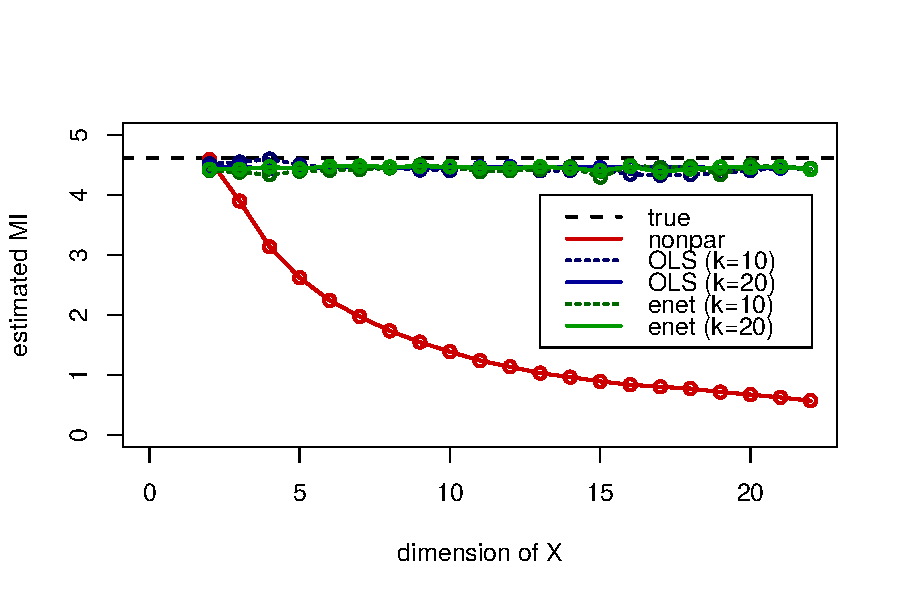
\includegraphics[scale = 0.8]{Figures/sim2a_fig1_edited.pdf}
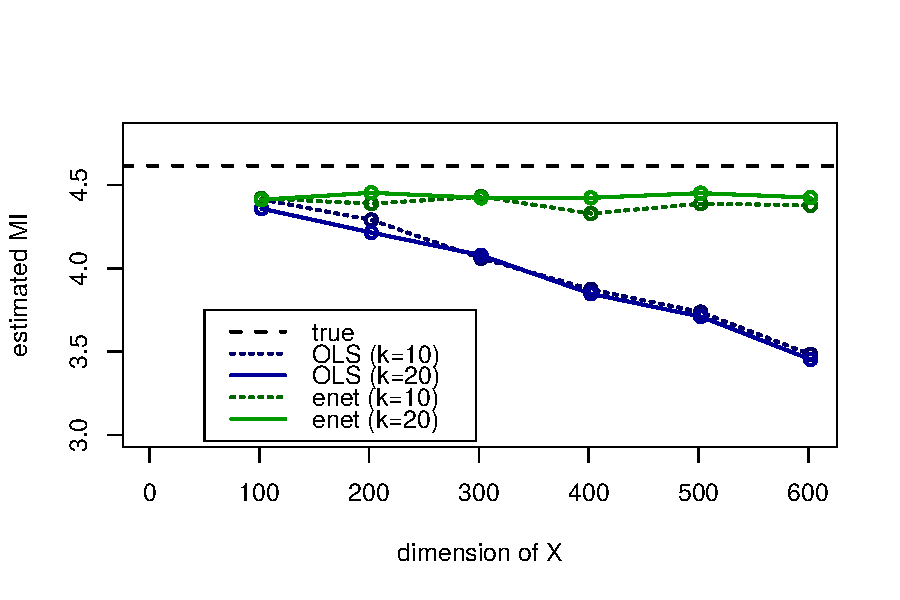
\includegraphics[scale = 0.8]{Figures/sim2a_fig3_edited.pdf}
\caption{Estimation of mutual information in simulated example.}
\label{fig:ch4_simulation}
\end{figure}

We will see additional examples in the next chapter, including a
simulation example involving a dense model.
